\chapter{正文排版建议以及一些示例}

\section{字体}
\label{sec:zi_ti_}


\section{标点符号}
\label{sec:biao_dian_fu_hao_}


\section{数学公式}
\label{sec:shu_xue_gong_shi_}

\subsection{公式环境建议}
\label{sub:gong_shi_huan_jing_jian_yi_}

在 \LaTeX{} 中插入数学公式有很多种方法, 包括行内公式和行间公式. 在这里根据我的使用经验, 给你提供一些建议.

%如果你想插入行内公式, 请使用\$公式\$, 虽然$\backslash($和$\backslash)$也能实现插入行内公式, 
如果你想插入行内公式, 请使用 \tilcode{\textbackslash(~\ldots~\textbackslash)}, 尽量不要使用 \tilcode{\$~\ldots~\$}.
前者是 \LaTeX{} 中的符号, 后者是 \TeX{} 中的符号. 尽管你可以在 \LaTeX{} 中两者都使用, 但是当你在公式里面
出现错误的时候, 前者不会给你太多费解的错误提示信息.

但是你也要注意, \tilcode{\textbackslash(~\ldots~\textbackslash)} 是个 \emph{fragile} 命令, 不能用在章节标题中.
当然如果你觉得你的公式不会出现错误, 你可以使用 \tilcode{\$~\ldots~\$}, 毕竟简洁清晰.

下面给出 \tilcode{\textbackslash(} 和 \tilcode{\textbackslash)} 在 \LaTeX{} 中的定义, 体会一下不同.
\begin{minted}{tex}
    \DeclareRobustCommand\({%
      \relax\ifmmode\@badmath\else$\fi}%
    \DeclareRobustCommand\){%
      \relax\ifmmode\ifinner$\else\@badmath\fi\else\@badmath\fi}%
\end{minted}

更多关于他们之间的讨论请参考脚注中提到的链接\footnote{\url{https://tex.stackexchange.com/questions/510/are-and-preferable-to-dollar-signs-for-math-mode}}.

如果你想插入行间公式, 请使用 \tilcode{\textbackslash begin\{equation\}~\dots~\textbackslash end\{equation\}}. 
尽管你可以使用 \tilcode{\$\$~\dots~\$\$} 或者是 \tilcode{\textbackslash[~\dots~\textbackslash]}, 但是
在你的论文中肯定是需要给公式编号的, 用 \tilcode{equation} 公式环境容易实现公式编号, 其他两个能不能
实现编号, 如何实现编号, 我不知道, 我也懒得去研究.

{\noindent
\begin{minipage}{.6\textwidth}
    \begin{minted}{tex}
        $$
            E = mc^{2}
        $$
    \end{minted}
\end{minipage}%
\begin{minipage}{.4\textwidth}
    $$
        E = mc^{2}
    $$
\end{minipage}
}

{\noindent
\begin{minipage}{.6\textwidth}
    \begin{minted}{tex}
        \[
            E = mc^{2}
        \]
    \end{minted}
\end{minipage}%
\begin{minipage}{.4\textwidth}
    \[
        E = mc^{2}
    \]
\end{minipage}
}

{\noindent
\begin{minipage}{.6\textwidth}
    \begin{minted}{tex}
        \begin{equation}
            E = mc^{2}
        \end{equation}
    \end{minted}
\end{minipage}%
\begin{minipage}{.4\textwidth}
        \begin{equation}
            E = mc^{2}
        \end{equation}
\end{minipage}
}

更多关于这方面的讨论请参考脚注中的链接\footnote{\url{https://tex.stackexchange.com/questions/503/why-is-preferable-to}}.

\subsection{公式排版建议}
\label{sub:gong_shi_pai_ban_jian_yi_}


\section{插图}
\label{sec:cha_tu_}

\section{表格}
\label{sec:biao_ge_}


\section{参考文献}
\label{sec:can_kao_wen_xian_}

本模板引入参考文献的命令是\tcodeinline{tex}{\cugthesisbib{bib_file_name}}.
会自动添加 ``参考文献'' 章节标题以及目录项, 所以不用你额外再写诸如\tcodeinline{tex}{\chapter{参考文献}}之类的代码.

\emph{bib\_file\_name} 是指你的参考文献数据库. 

关于参考文献数据库你可以自己手动录入, 也可以使用工具自动生成. 比如说 Zotero, JabRef, Mendeley 这些参考文献
管理工具.
% 如图\ref{fig:bibtoolexport}所示是我用 Zotero 导出文献引用数据.
%\begin{tfig}{Zotero导出参考文献引用数据}{fig:bibtoolexport}
    %\begin{minipage}{.66\textwidth}
        %\includegraphics[width=\textwidth]{./imgs/zoteroexport1.png}
    %\end{minipage}%
    %\begin{minipage}{.33\textwidth}
        %\includegraphics[width=\textwidth]{./imgs/zoteroexportbibtex.png}
    %\end{minipage}
%\end{tfig}

你也可以在下载参考文献的时候下载其对应的 cite key, 如图\ref{fig:bibcitekey}. 
\begin{tfig}{文献 bibtex}{fig:bibcitekey}
    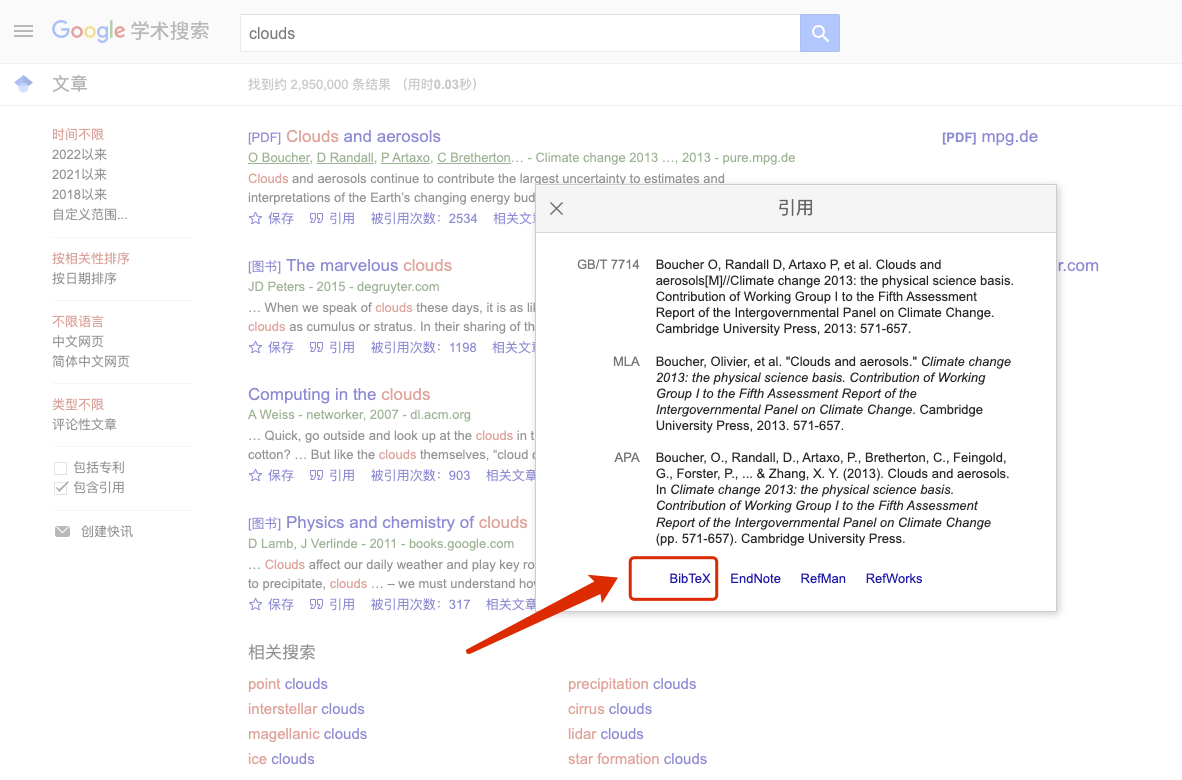
\includegraphics[width=.7\textwidth]{./imgs/cite_bib.png}
\end{tfig}

\endinput